%----------------------------------------------------------------------------------------
%	PACKAGES AND THEMES
%----------------------------------------------------------------------------------------
\documentclass[aspectratio=169,xcolor=dvipsnames,8pt]{beamer}
\usetheme{Simple}
\usefonttheme[onlymath]{serif}
\usepackage{hyperref}
\usepackage{graphicx} % Allows including images
\usepackage{booktabs} % Allows the use of \toprule, \midrule and \bottomrule in tables
\usepackage{tikz}
\newcommand{\beq}{\begin{equation}}
\newcommand{\eeq}{\end{equation}}
\newcommand{\bes}{\begin{split}}
\newcommand{\ees}{\end{split}}
\newcommand{\BB}{\textbf{B}}
\newcommand{\jj}{\textbf{j}}
\newcommand{\x}{\times}
\newcommand{\ii}{\iota}
\newcommand{\iotaa}{\bar{\iota}}
\newcommand{\dd}{\partial}
\graphicspath{{./Figures/}}  

\setbeamersize{text margin left=14mm,text margin right=14mm}


%----------------------------------------------------------------------------------------
%	TITLE PAGE
%----------------------------------------------------------------------------------------

% The title
\title[Summary]{Numerical study of the effect of secondary electron emission on the dynamics of electron clouds in gyrotron guns}

\author[S.Guinchard] {S. ~Guinchard$^{1}$, G. ~Le Bars$^{2}$}
\institute[SPH] % Your institution may be shorthand to save space
{
    % Your institution for the title page
    $^1$ Ecole Polytechnique Fédérale de Lausanne (EPFL), Physics Section (SPH), CH-1015 Lausanne, Switzerland\\
    $^2$ Ecole Polytechnique Fédérale de Lausanne (EPFL), Swiss Plasma Center (SPC), CH-1015 Lausanne, Switzerland\\
    \vspace{1cm}
}
\date{\today} % Date, can be changed to a custom date

% Backgorund
\usebackgroundtemplate%
{%
    \includegraphics[width=\paperwidth,height=\paperheight]{Figures/Beamer_background}%
}



%----------------------------------------------------------------------------------------
%	PRESENTATION SLIDES
%----------------------------------------------------------------------------------------

\begin{document}

\begin{frame}
    % Print the title page as the first slide
    \titlepage
\end{frame}

% %------------------------------------------------
%%%%%%%%%%%%%%%%%%%%%%

\begin{frame}{IIEE - implementation}

\begin{itemize}


\item{Recall: electronic yield $\gamma(E) = \Lambda_{exp}*\frac{dE_{ions}}{dx}$ }
\item{Ion Induced Electrons have been modeled using a Poisson Law}
\vspace{1cm}
\item{$P(x=k) = e^{-\lambda}\frac{\lambda^k}{k!} =  e^{-\gamma(E_i)}\frac{\gamma(E_i)^k}{k!} $}
\end{itemize}
\end{frame}


%-------------------------------------------------
%%%%%%%%%%%%%%%%%%%%%%

 \begin{frame}{Module tests}
     \begin{columns}[c] % The "c" option specifies centered vertical alignment while the "t" option is used for top vertical alignment

         \column{.5\textwidth} % Left column and width
	\begin{itemize}


		\item{Vertical slice of He ions impinging on stainless steel electrode\\
			\begin{itemize}
		
				\item{Potential bias: $\Delta\phi = 20kV$}
				\item{Electrode radial positions: $r_a = 10^{-3}m$, $r_b = 10^{-2}m$ }
				\item{Acquired energy: $E\propto \Delta \phi \log(r/r_a)/\log(r_b/r_a)$} 
				\end{itemize}}
				
						
	\end{itemize}

         \column{.5\textwidth} % Right column and width
		\begin{figure}[h!]
		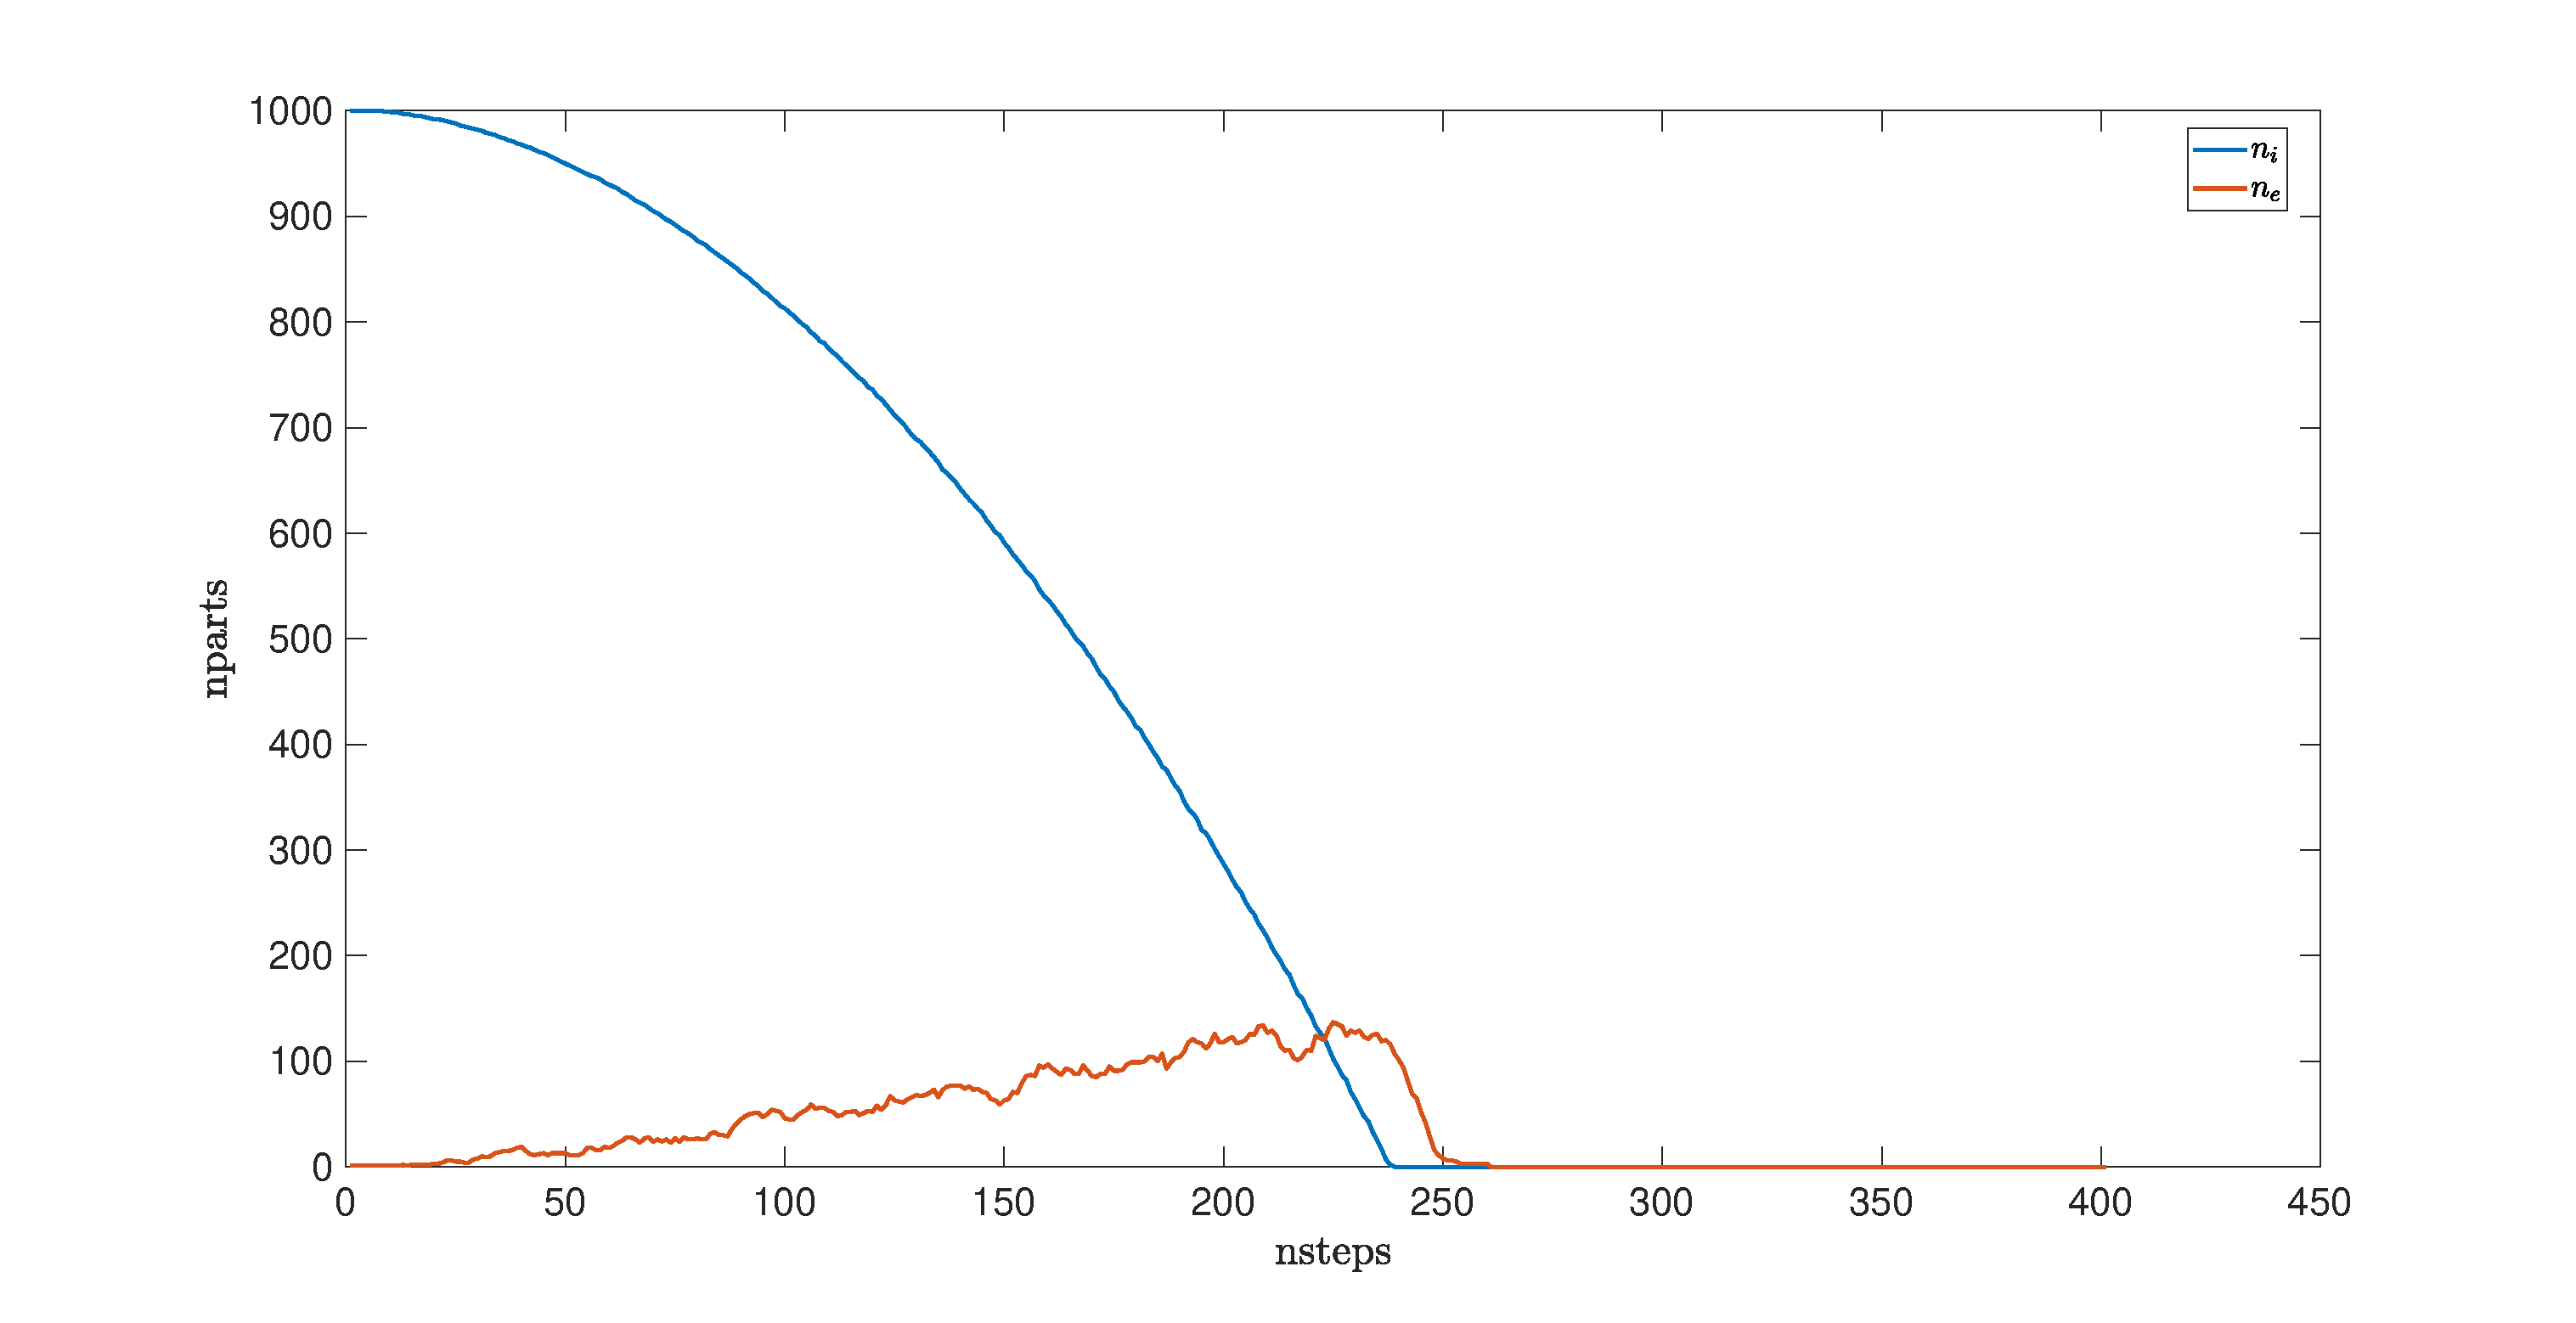
\includegraphics[width=1 \textwidth]{vertslice.eps}
		\caption{\label{img1}  Particles number as function of time}
		\end{figure}
     \end{columns}
\end{frame}
% %------------------------------------------------
%%%%%%%%%%%%%%%%%%%%%

  \begin{frame}{Module tests}
     \begin{columns}[c] % The "c" option specifies centered vertical alignment while the "t" option is used for top vertical alignment

         \column{.5\textwidth} % Left column and width
	\begin{itemize}


		\item{Horizontal slice of He ions impinging on stainless steel electrode\\
			\begin{itemize}
		
				\item{Potential bias: $\Delta\phi = 20kV$}
				\item{Electrode radial positions: $r_a = 10^{-3}m$, $r_b = 10^{-2}m$ }
				\item{Acquired energy: $E\propto \Delta \phi \log(r/r_a)/\log(r_b/r_a)$} 
				\item{Yield prediction: Slice 1: $\gamma =0.96$, Slice 2: $\gamma = 1.33$}
				\item{Obtained yield: Slice 1: 967 $e^{-}$ for 1000 lost ions}
				\item{Slice 2: 1325 for 1000 ions : Relative error $\propto 1e-3$}
				\end{itemize}}
				
						
	\end{itemize}

         \column{.5\textwidth} % Right column and width
		\begin{figure}[h!]
		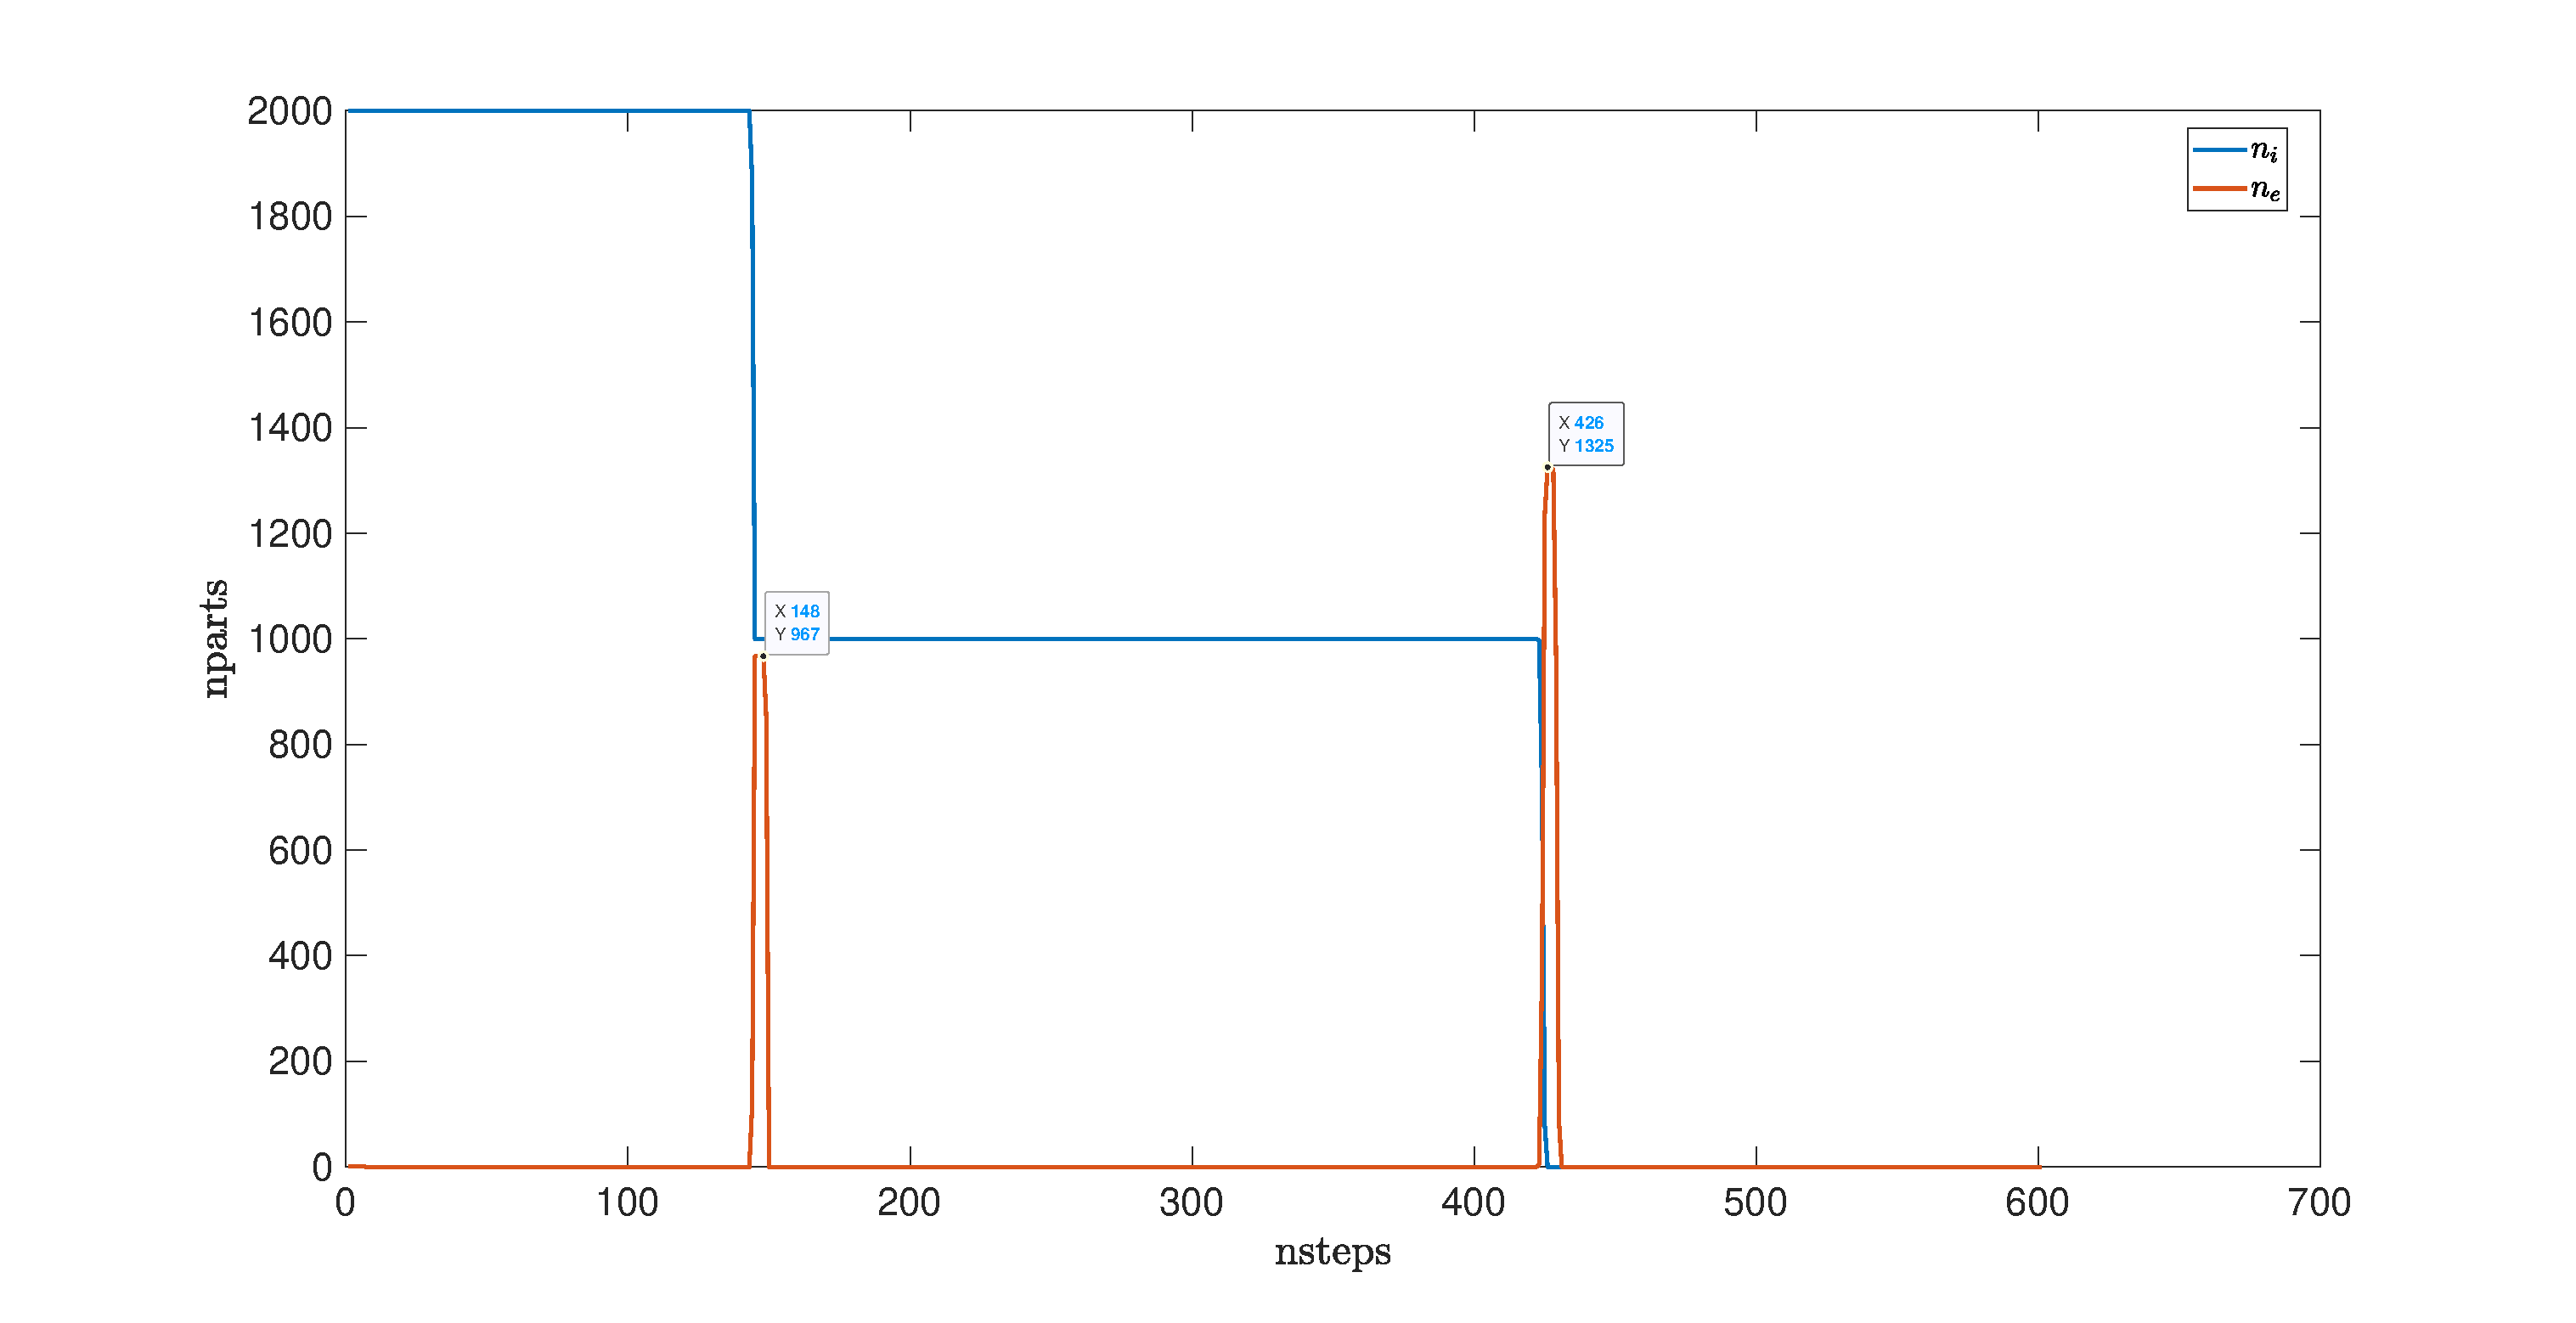
\includegraphics[width=1 \textwidth]{flatslice.eps}
		\caption{\label{img1} Particles number as function of time}
		\end{figure}
     \end{columns}
\end{frame}
% %------------------------------------------------
%%%%%%%%%%%%%%%%%%%%
  \begin{frame}{Module tests - TREX extrude geometry}
     \begin{columns}[c] % The "c" option specifies centered vertical alignment while the "t" option is used for top vertical alignment

         \column{.5\textwidth} % Left column and width
	\begin{itemize}


		\item{Rectangle of incident ions at peak of cloud density \\
			\begin{itemize}
		
				\item{5000 incident ions}
				\item{Zero initial energy}
				\item{End of simulation: +570 electrons remaining}
				\item{$\sim 10 \%$ of incident ions number}
				\end{itemize}}
				
						
	\end{itemize}

         \column{.5\textwidth} % Right column and width
		\begin{figure}[h!]
		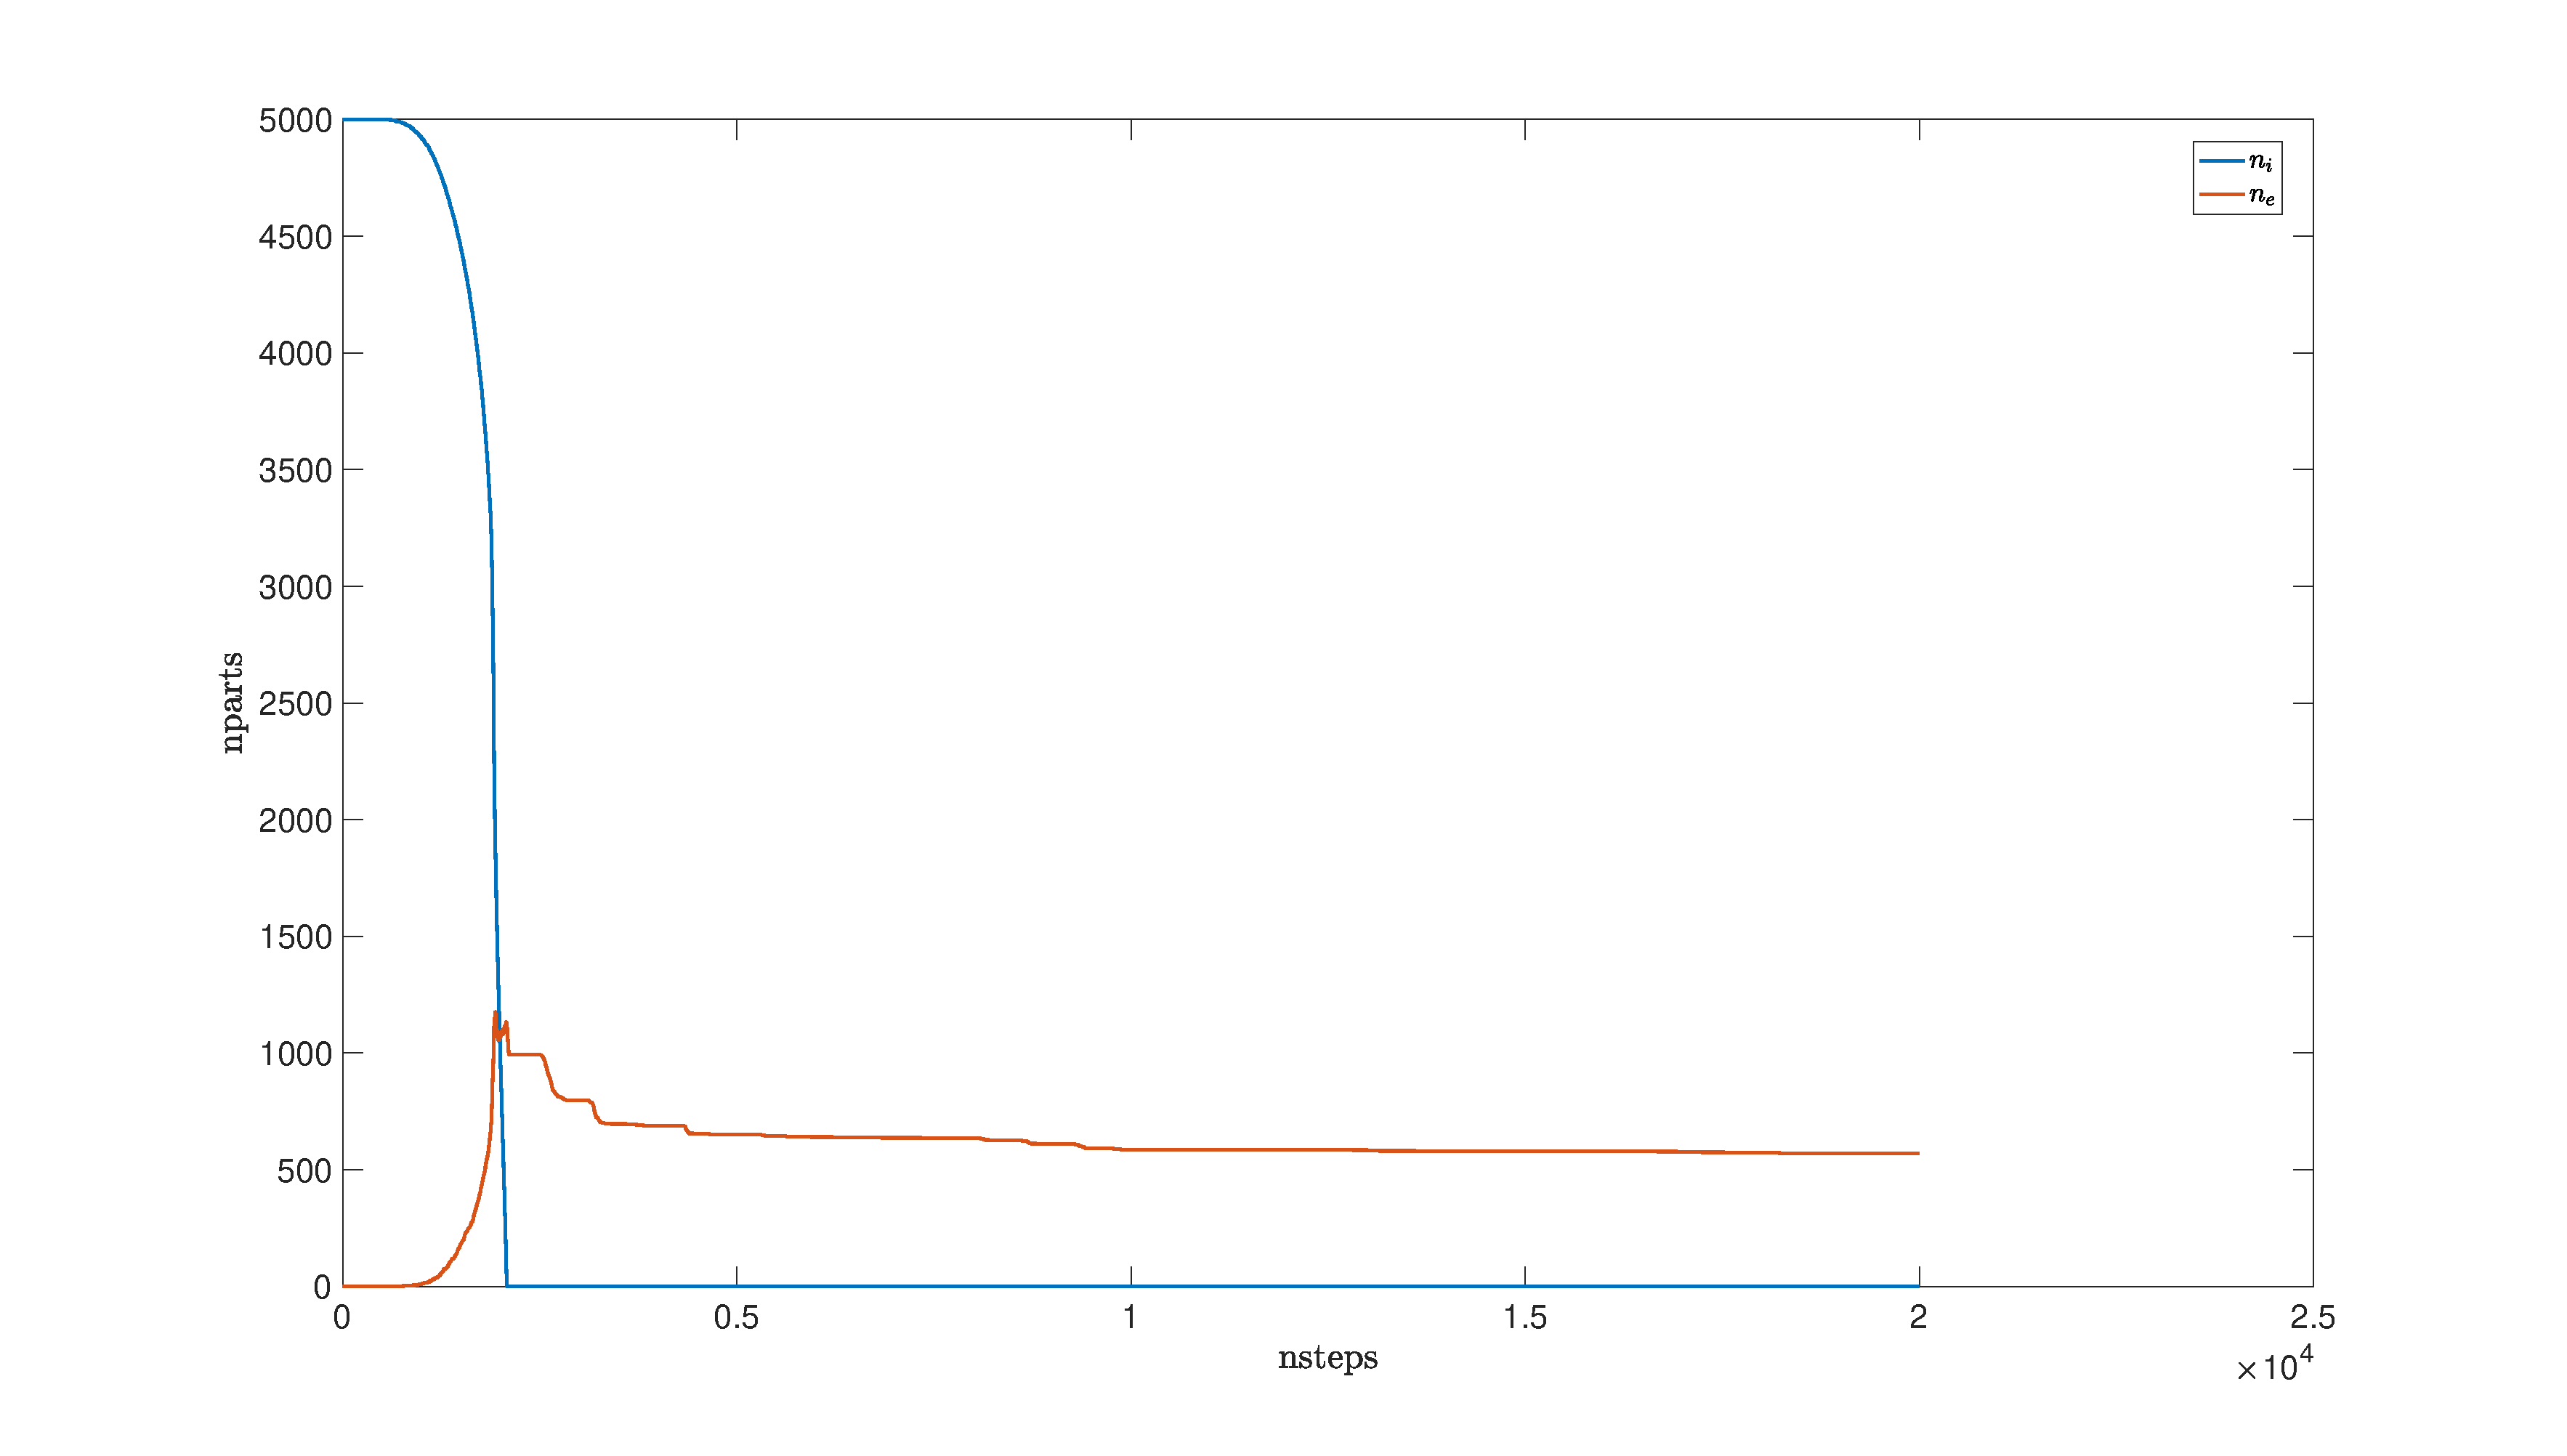
\includegraphics[width=1 \textwidth]{nparts_peak_density.eps}
		\caption{\label{img1} Particles number as function of time}
		\end{figure}
     \end{columns}
\end{frame}

% %------------------------------------------------
%%%%%%%%%%%%%%%%%%%%
  \begin{frame}{Module tests - TREX extrude geometry}
     \begin{columns}[c] % The "c" option specifies centered vertical alignment while the "t" option is used for top vertical alignment

         \column{.5\textwidth} % Left column and width
	\begin{itemize}


		\item{Rectangle of incident ions around whole cloud \\
			\begin{itemize}
		
				\item{5000 incident ions}
				\item{Zero initial energy}
				\item{End of simulation: $\sim 700$ electrons remaining}
				\item{$ \sim 14 \%$ of incident ions number}
				\end{itemize}}
				
						
	\end{itemize}

         \column{.5\textwidth} % Right column and width
		\begin{figure}[h!]
		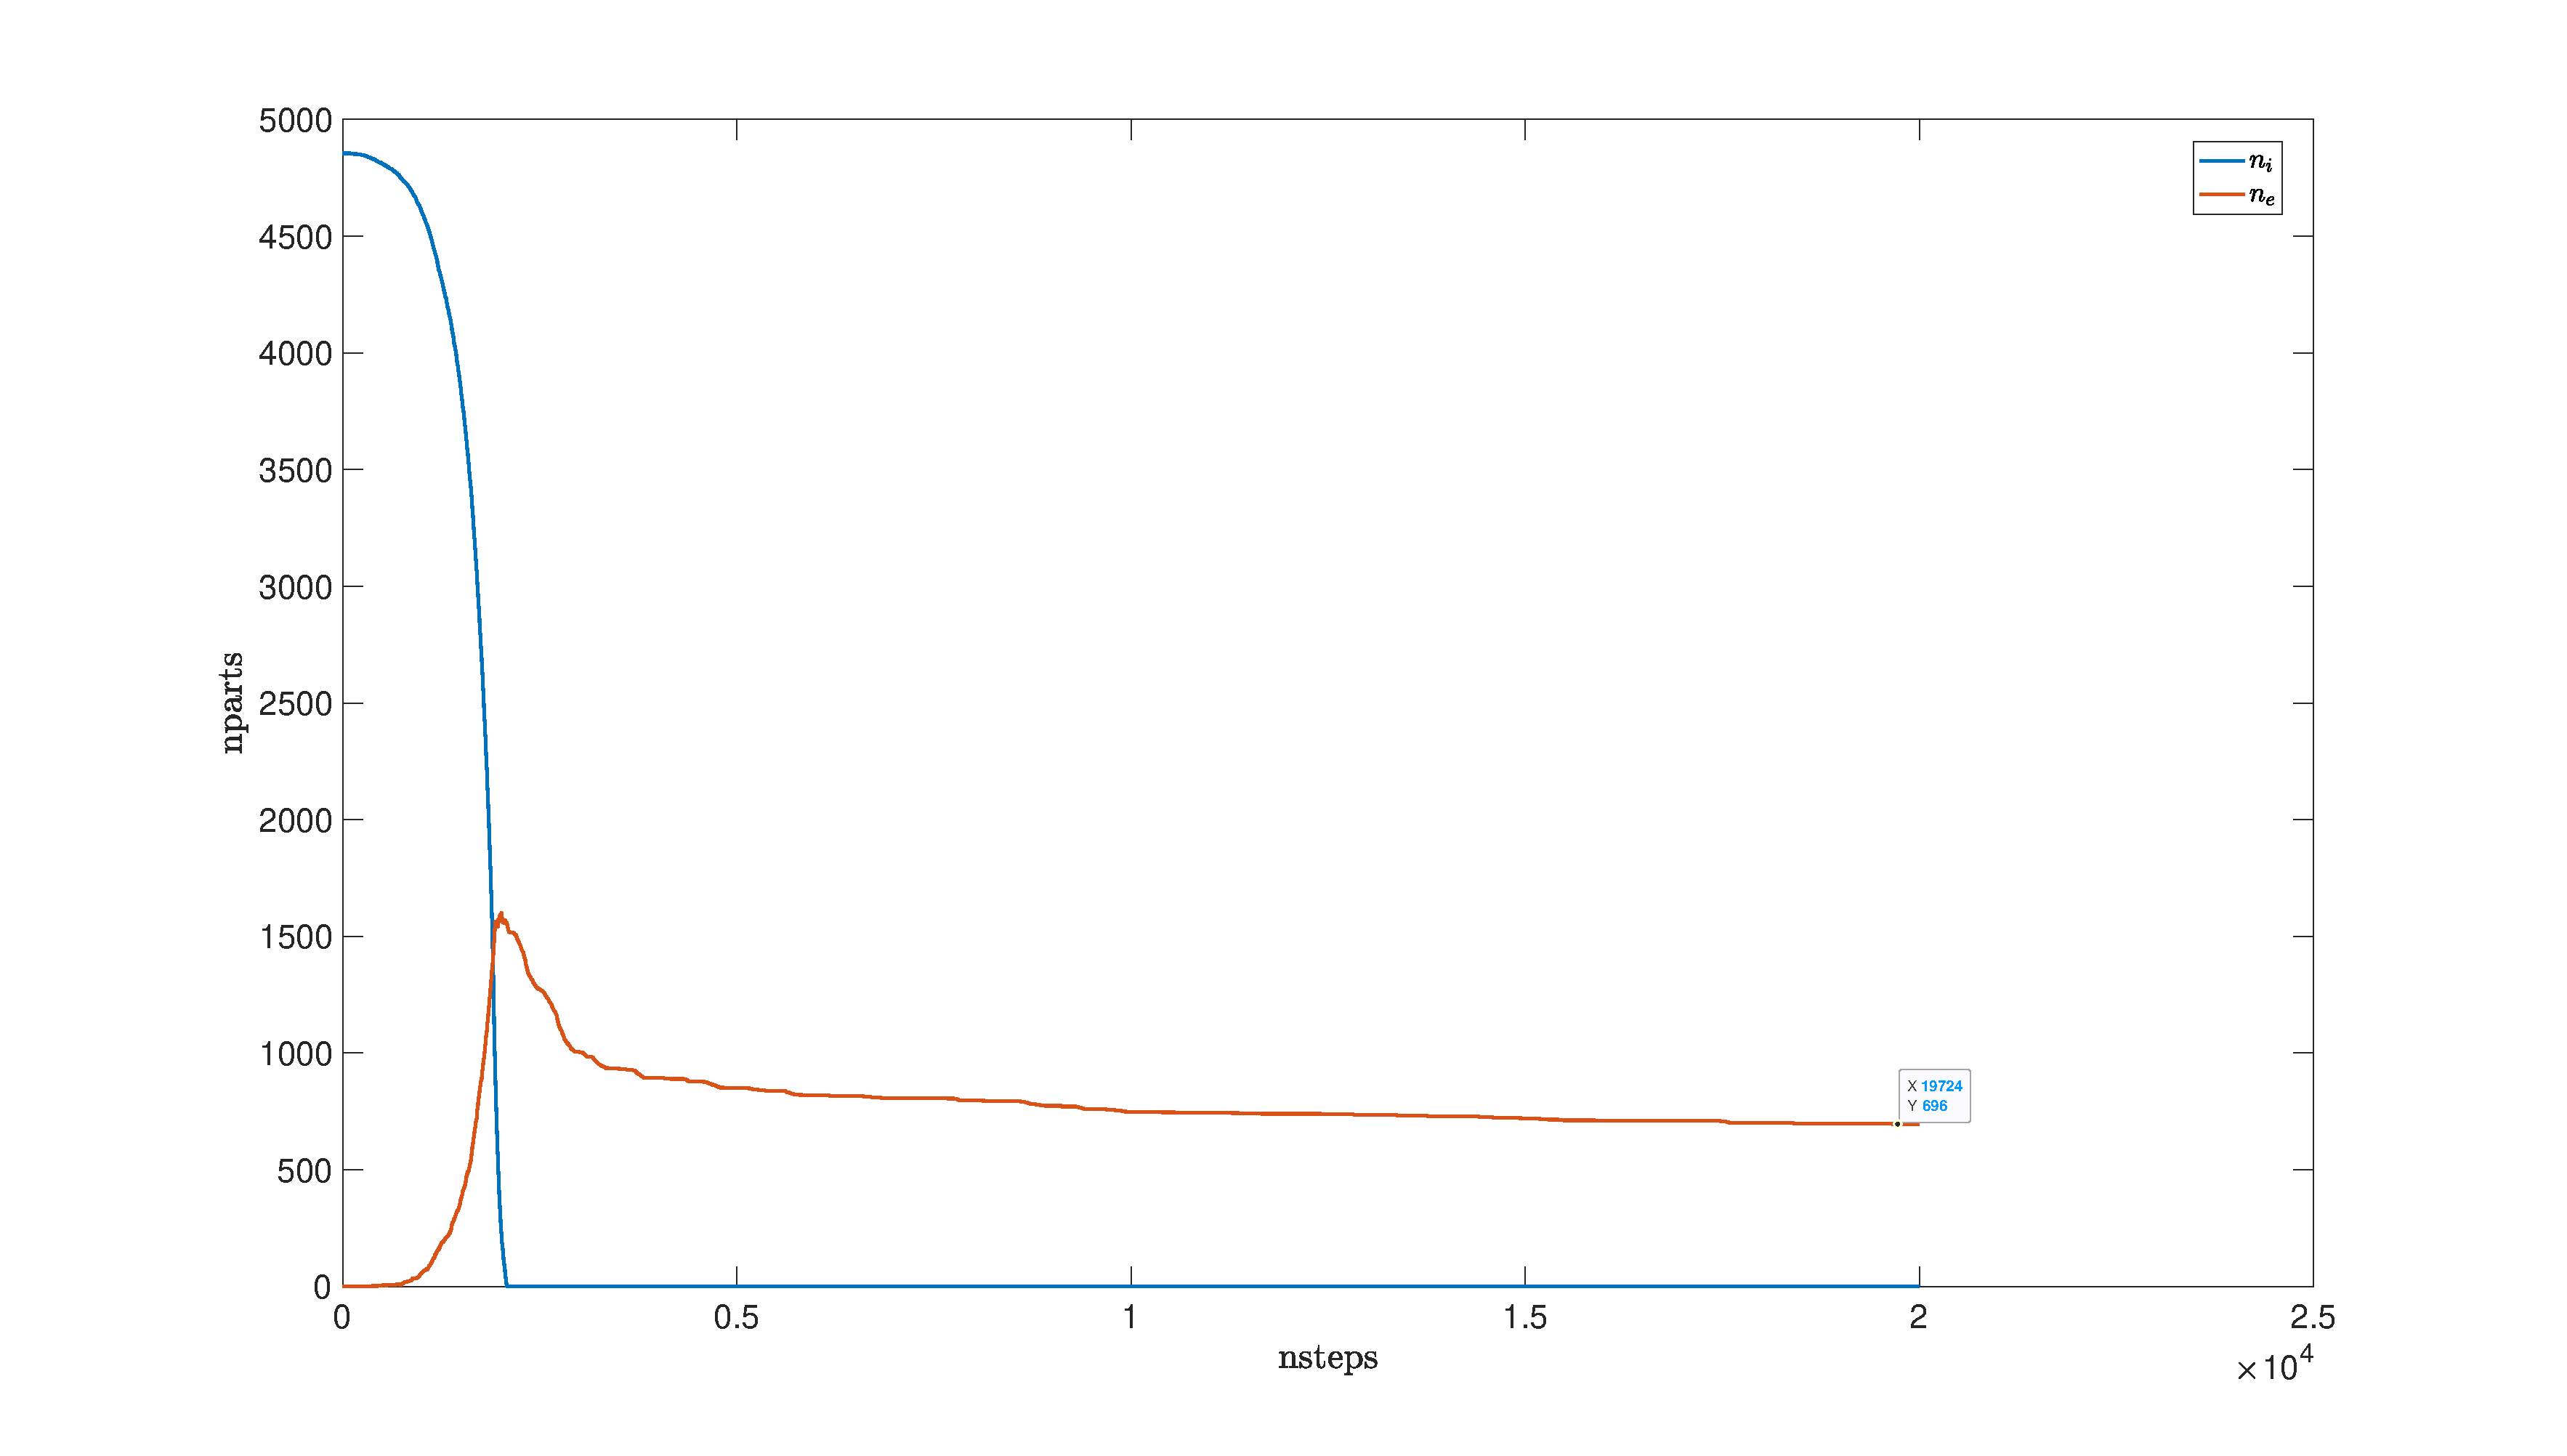
\includegraphics[width=1 \textwidth]{parts_number_wholde_cloud}
		\caption{\label{img1} Particles number as function of time}
		\end{figure}
     \end{columns}
\end{frame}


%%%%%%%%%%%%%%%%%%%%

\end{document}

